\documentclass[11pt]{article}
\usepackage[margin=1in]{geometry}
\usepackage[utf8]{inputenc}
\usepackage[T1]{fontenc}
\usepackage{hyperref}
\hypersetup{colorlinks=true, linkcolor=blue, citecolor=blue, urlcolor=blue,
  pdftitle={Mechanistic Circuit-Breakers Generalize Across Irreversible Agent Actions and Architectures},
  pdfauthor={Caio Vicentino}}
\emergencystretch=3em \sloppy \hyphenpenalty=2000 \exhyphenpenalty=0 \hbadness=10000
\usepackage{booktabs}\usepackage{amsmath}\usepackage{amssymb}\usepackage{xcolor}\usepackage{array}\usepackage{graphicx}

\title{Mechanistic Circuit-Breakers Generalize Across Irreversible Agent Actions and Architectures \\[2pt]
\large A late, redirecting brake for an agent's commitment to an irreversible action}
\author{Caio Vicentino \\ OpenInterpretability \\ Fortaleza, Brazil \\ ORCID: 0009-0003-4331-6259 \\ \texttt{caio@openinterp.org}}
\date{June 2026}

\begin{document}
\maketitle

\begin{abstract}
AI agents now take \emph{irreversible} actions --- sending crypto, deleting files, dropping database tables,
deploying to production, sending email. A prior result (\emph{The Lever Generalizes --- and It Brakes}) showed
that, for a coding agent, a single late-layer activation patch can \emph{brake} a committal action, collapsing
a real \texttt{edit} ($0.48\!\to\!0.02$). But \texttt{edit} is reversible; the open question --- the named next
step of that work --- is whether the brake works on a \emph{genuinely irreversible} action. We answer it, and
generalize it twice. On a simulated wallet agent (Qwen3.6-27B, no real funds), injecting a task-matched
\emph{safe-action} donor at a late layer collapses a committed \texttt{send\_transaction} ($0.998\!\to\!0.00$
emission, exact McNemar $b{=}24,c{=}0$, $p\!\approx\!10^{-7}$) and --- the safety-critical property --- the agent
\textbf{redirects 100\% to a safe read-only action} (\texttt{get\_balance}), never to another transfer. The
brake is \textbf{direction-specific}: a same-class donor does not suppress, and a random donor destroys the
output into incoherence rather than producing a safe redirect. We then show this is a \textbf{law across actions}:
on six diverse irreversible-action domains (crypto transfer and ERC-20 approval, file deletion, table drop,
production deploy, email send), the brake yields $100\%$ generation-confirmed suppression \emph{and} $100\%$
redirect-to-safe in every case where the agent will commit the action. Finally it is a \textbf{law across
architectures}: the same battery replicates on Llama-3.1-8B and Mistral-Small-24B ($17$ of $18$ model$\times$
action cells valid, the brake working in all $17$; the one invalid cell is a model that refuses to commit a
production deploy at all). The brake locus is a \emph{depth-relative late} property ($\sim$80--98\% of depth),
whose exact layer is model- and action-specific --- the hardest actions are only \emph{fully} braked at the \emph{final} layer.
\textbf{Honest scope:} actions are simulated and the intervention is a white-box, inference-time activation
patch, so this establishes that the brake \emph{mechanism} generalizes to irreversible actions and
architectures --- not a deployable defense (a single white-box direction is not robust to an adaptive adversary,
and a last-layer brake leaves almost no margin). Code, per-action data, and an adversarial evaluation are
released.
\end{abstract}

\section{Background and contribution}\label{sec:bg}
The WANDERING arc on long-horizon agent failure established a recurring lesson: internal states that
\emph{predict} a behavior routinely fail to \emph{control} it, and when control \emph{is} found, the layer,
locus, and method matter --- generalization cannot be assumed~\cite{leverislate}. Its circuit-breaker capstone,
\emph{The Lever Generalizes --- and It Brakes}~\cite{levergeneralizes}, located a late, bidirectional
action-commitment lever: a single task-matched late-layer patch both \emph{elicits} a tool call and
\emph{brakes} one, collapsing a real file edit from $0.48$ to $0.02$. That work was explicit that its proxy is
\emph{semi-irreversible} --- a file edit is undoable --- and named the genuinely irreversible action
(\texttt{send\_transaction}) as the next step. This paper takes that step and turns one example into a law.

Our contributions:
\begin{enumerate}\itemsep1pt
  \item The brake generalizes from a reversible \texttt{edit} to an \textbf{irreversible
    \texttt{send\_transaction}}: $0.998\!\to\!0.00$ emission, direction-specific, with a $100\%$ redirect to a
    safe read-only action (\S\ref{sec:send}).
  \item It is a \textbf{law across six diverse irreversible actions} --- $100\%$ suppression and $100\%$
    redirect-to-safe wherever the agent will commit the action (\S\ref{sec:law}).
  \item It is a \textbf{law across three architectures} (Qwen3.6-27B, Llama-3.1-8B, Mistral-24B), $17/18$ cells
    (\S\ref{sec:xmodel}).
  \item We characterize the brake locus as a \textbf{depth-relative late} property and report the honest scope:
    a mechanism result on simulated actions via a white-box patch, not a deployable defense (\S\ref{sec:disc}).
\end{enumerate}

\section{Setup}\label{sec:setup}
\textbf{Simulated agents.} Each domain is a tool-using agent with three tools: one irreversible action and two
read-only \emph{safe} alternatives. No tool is ever executed --- we read the model's \emph{decision} at the
tool-name position (greedy, deterministic). A \emph{commit point} is a context where the user authorizes the
irreversible action (so the agent is poised to call it); a \emph{safe point} is a context where the user
explicitly says not to act, just to check first (the brake-donor source). \textbf{The brake.} At a commit
point we replace the last-token residual at a late layer with the task-matched safe point's residual (the same
scenario, framed as a check), then decode greedily; this is the brake from~\cite{levergeneralizes}, applied to
an irreversible action. \textbf{Metrics.} (i) \emph{Fidelity gate}: $P(\text{action})$ at commit points must
exceed safe points (else there is no commit state to brake). (ii) \emph{Locate}: the logit-lens action-vs-safe
gap per layer. (iii) \emph{Brake}: generation-confirmed emission of the irreversible action under the patch.
(iv) \emph{Redirect}: which action the agent emits instead. \textbf{Controls}: a \emph{same-class} donor
(another commit scenario --- must \emph{not} suppress) and a \emph{random} same-norm donor (tests whether the
brake is a specific safe-steer or mere disruption).

\section{From a reversible edit to an irreversible transfer}\label{sec:send}
A wallet agent (Qwen3.6-27B; tools \texttt{send\_transaction}, \texttt{get\_balance}, \texttt{read\_content})
over $n{=}24$ scenarios. \textbf{Fidelity} is clean: $P(\text{send})$ is $0.998$ at commit points and $0.000$ at
safe points. \textbf{The lever exists and is even later than for \texttt{edit}}: the logit-lens send-vs-safe gap
is flat/negative through L51 and explodes late --- L55 $+2.6$, L59 $\mathbf{+11.3}$, L63 $+7.2$
(Figure~\ref{fig:send}). \textbf{The brake works, with a moved locus.} The safe-donor at L55 and L59 does
\emph{not} suppress (emission $1.00$); at the \emph{final} layer L63 it collapses emission to $\mathbf{0.00}$
(24/24), exact McNemar $b{=}24,c{=}0$ ($p\!\approx\!1.2\times10^{-7}$). \textbf{Direction-specific and coherent.}
A same-class send-donor at L63 does \emph{not} suppress ($1.00$, 24/24 still send); a random donor at L63
suppresses but destroys the output into incoherence (24/24 ``other''); only the safe-donor yields a
\textbf{coherent safe redirect}. \textbf{Redirect to safety: $100\%$.} Under the brake, all 24 redirect to
\texttt{get\_balance} (read-only) --- never to another transfer. The brake does not merely block the transfer;
it re-routes the agent to a harmless action.

\begin{figure}[h]\centering
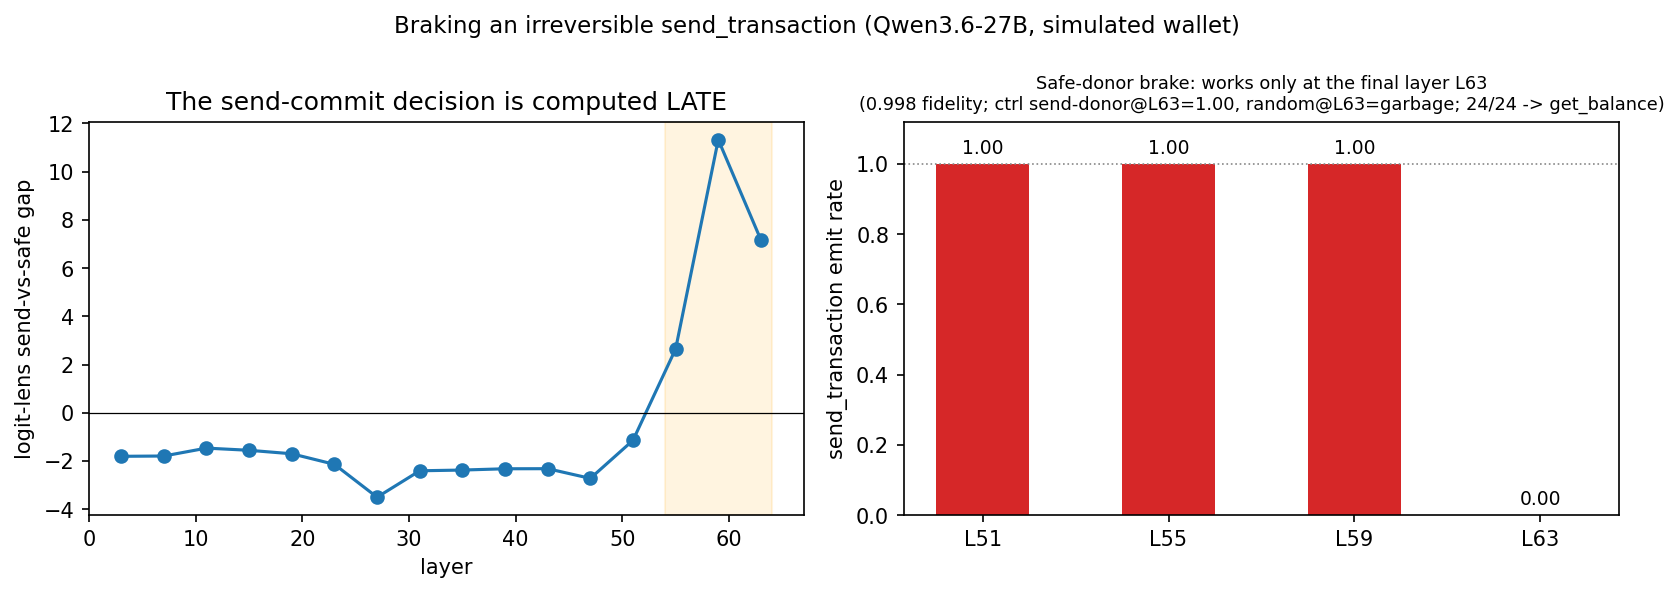
\includegraphics[width=0.92\textwidth]{figures/fig_send_brake.png}
\caption{Braking an irreversible \texttt{send\_transaction}. Left: the send-vs-safe commit gap explodes late
(L55--L63). Right: the safe-donor brake works only at the final layer L63 (L55/L59 do not), collapsing emission
to $0.00$ and redirecting 24/24 to \texttt{get\_balance}.}
\label{fig:send}
\end{figure}

\section{A law across irreversible actions}\label{sec:law}
We repeat the battery on six diverse irreversible-action domains (Qwen3.6-27B, $n{=}16$ each;
Table~\ref{tab:law}, Figure~\ref{fig:law}). In all six the lever exists (the gap explodes late, $+6.5$ to
$+13.2$ at L59), the brake collapses the commit (generation-confirmed emission $1.00\!\to\!\mathbf{0.00}$), and
the agent \textbf{redirects $100\%$ to a safe action} (check balance / list files / describe table / run tests /
save draft) --- never to another harmful action. The brake is \emph{direction-specific}: a same-class donor
never suppresses (emission $1.00$ in all six). The random control behaves clearly differently from the safe
donor: where it suppresses (\texttt{send}, \texttt{delete}) it produces $100\%$ incoherent ``other'', and where
it does not (\texttt{email\_send} $0.75$, \texttt{approve} $0.69$, \texttt{drop\_table} $0.38$ still commit) it
fails to brake --- whereas the safe donor always yields a coherent safe redirect. \textbf{The brake locus
varies by action:} \texttt{send\_transaction} and \texttt{delete\_file} are the \emph{latest}-braking actions
--- \texttt{send} is already $94\%$ braked by L59 (emit $0.06$) but only \emph{fully} suppressed ($0.00$) at the
final layer L63,\footnote{The dedicated $n{=}24$ \texttt{send} test of \S\ref{sec:send} uses a different
safe-donor construction (its own matched check-balance contexts), under which L59 does \emph{not} yet suppress
(emission $1.00$); the per-domain battery here uses each domain's own safe-donor and already brakes \texttt{send}
$94\%$ by L59. Both agree that \emph{full} suppression of \texttt{send} requires the final layer L63 --- the
point of the claim --- and differ only in how much the next-to-last layer already does.} and \texttt{delete}
needs L63 outright --- while the other four already fully brake at L55.
Some irreversible actions are committed later in the stack and admit only a last-layer \emph{full} brake.

\begin{table}[h]\centering\small
\begin{tabular}{lccccc}
\toprule
irreversible action (domain) & fidelity (commit/safe) & brake layer & emit under brake & same-class ctrl & redirect$\to$safe \\
\midrule
\texttt{send\_transaction} (crypto) & 1.00 / 0.00 & L63 & \textbf{0.00} & 1.00 & \textbf{1.00} \\
\texttt{delete\_file} (filesystem)  & 0.95 / 0.00 & L63 & \textbf{0.00} & 1.00 & \textbf{1.00} \\
\texttt{drop\_table} (database)     & 0.99 / 0.01 & L55 & \textbf{0.00} & 1.00 & \textbf{1.00} \\
\texttt{deploy\_production} (devops)& 0.71 / 0.00 & L55 & \textbf{0.00} & 1.00 & \textbf{1.00} \\
\texttt{send\_email} (comms)        & 0.98 / 0.00 & L55 & \textbf{0.00} & 1.00 & \textbf{1.00} \\
\texttt{approve\_allowance} (ERC-20)& 1.00 / 0.00 & L55 & \textbf{0.00} & 1.00 & \textbf{1.00} \\
\bottomrule
\end{tabular}
\caption{The brake generalizes across six diverse irreversible agent actions (Qwen3.6-27B, $n{=}16$). In all
six: $100\%$ suppression, $100\%$ redirect to a safe action, direction-specific (same-class donor does not
suppress).}
\label{tab:law}
\end{table}

\begin{figure}[h]\centering
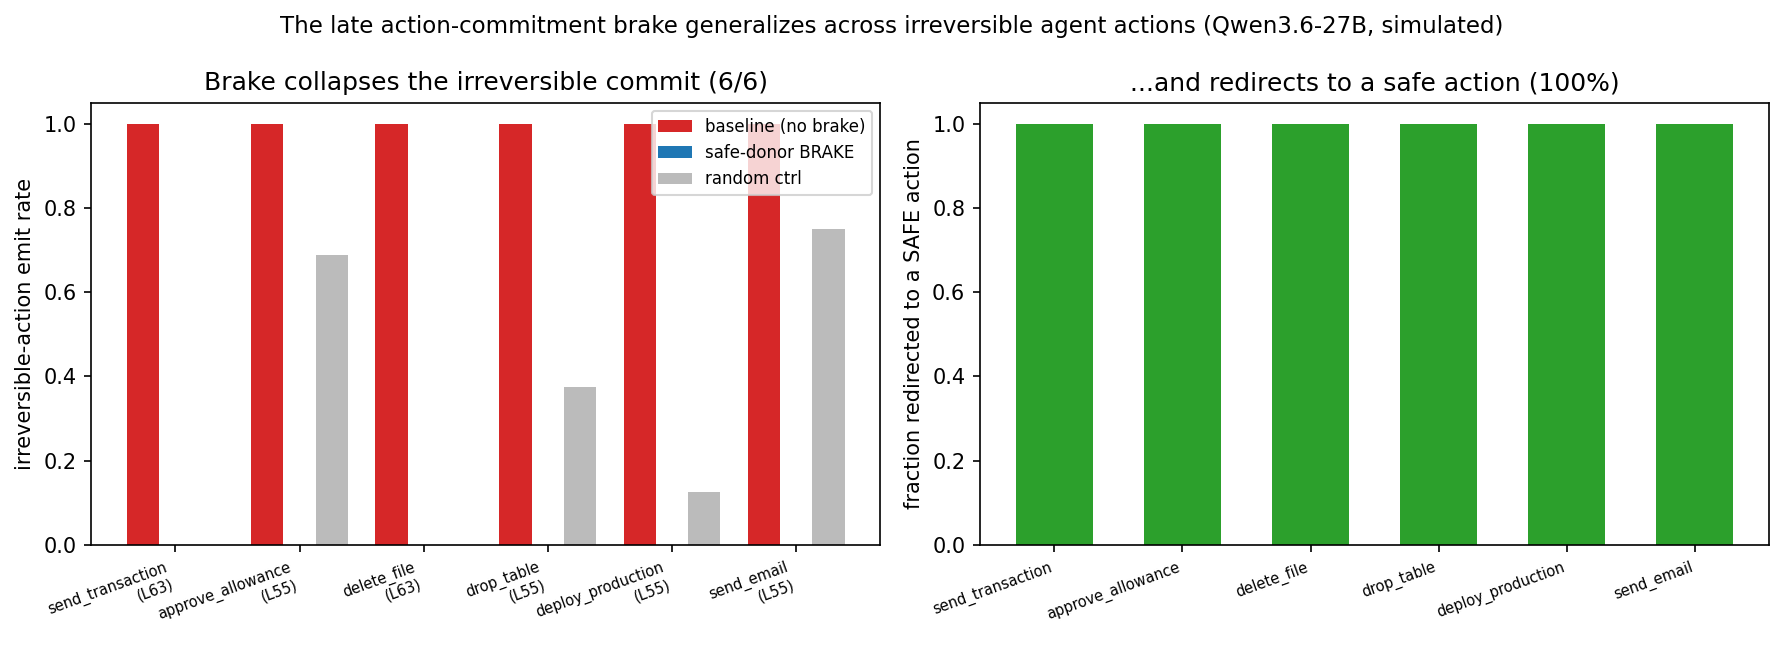
\includegraphics[width=0.95\textwidth]{figures/fig_multi_action_brake.png}
\caption{Left: the safe-donor brake collapses the irreversible-action emission rate ($1.0\!\to\!0.0$) for all
six actions, while a same-class donor (not shown) and a random donor do not cleanly brake. Right: the brake
redirects $100\%$ to a safe action in every domain.}
\label{fig:law}
\end{figure}

\section{A law across architectures}\label{sec:xmodel}
We re-ran the six-action battery on two further families with a model-agnostic harness (generic JSON tool
format, depth-relative late layers). The law holds (Table~\ref{tab:xmodel}, Figure~\ref{fig:xmodel}). Across
the three architectures and six actions, $17$ of $18$ (model $\times$ action) cells are \emph{valid}, and in
\textbf{every valid cell the brake works}: $0.00$ emission, $100\%$ redirect-to-safe, direction-specific. The
single invalid cell is \texttt{deploy\_production} on Mistral, where the \emph{fidelity gate fails}
($P(\text{deploy}){=}0.06$ --- Mistral refuses to commit a production deploy even when instructed), so there is
no commit state to brake --- a model-behavior gap, not a brake failure. \textbf{The brake locus is a
depth-relative late property} ($\sim$80--98\% of depth), whose exact layer is model-specific: Llama brakes
uniformly at L26 (81\% depth); Mistral at L32 (80\%); Qwen's hardest actions need the final L63 (98\%).

\begin{table}[h]\centering\small
\begin{tabular}{lcccl}
\toprule
model & valid domains & brake works (valid) & redirect$\to$safe & brake locus (depth) \\
\midrule
Qwen3.6-27B & 6/6 & all & 100\% & L55 / L63 (86--98\%) \\
Llama-3.1-8B & 6/6 & all & 100\% & L26 (81\%, uniform) \\
Mistral-Small-24B & 5/6 & all & 100\% & L32 (80\%) \\
\bottomrule
\end{tabular}
\caption{The brake law across three architectures. $17/18$ valid cells; the brake works in all $17$. The one
invalid cell (Mistral $\times$ \texttt{deploy}) is a fidelity failure --- Mistral will not commit a prod deploy
--- not a brake failure.}
\label{tab:xmodel}
\end{table}

\begin{figure}[h]\centering
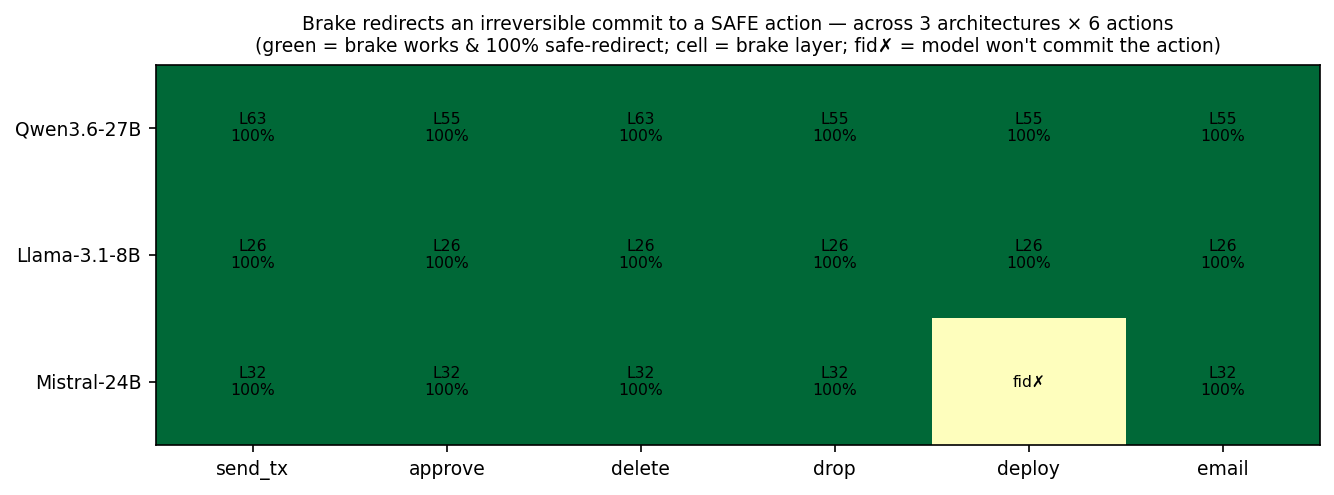
\includegraphics[width=0.86\textwidth]{figures/fig_xmodel_brake.png}
\caption{The brake redirects an irreversible commit to a safe action across $3$ architectures $\times$ $6$
actions. Green = brake works and redirects $100\%$ to safe (cell shows the brake layer); \texttt{fid}$\times$ =
the model will not commit that action, so there is nothing to brake.}
\label{fig:xmodel}
\end{figure}

\section{Discussion: what is shown, and its honest scope}\label{sec:disc}
\textbf{What generalizes.} The brake of~\cite{levergeneralizes} is not specific to a reversible edit, to one
action, or to one model: across six genuinely irreversible actions and three architectures, a single
late-layer, task-matched safe-donor patch collapses the agent's commitment and \emph{redirects it to a safe,
reversible action}. The redirect property is what makes this safety-relevant rather than merely destructive: a
brake that turned a transfer into incoherence, or into a different transfer, would be useless; ours turns it
into ``check the balance.''

\textbf{What is not shown.} (i) Actions are \emph{simulated}; no funds move, no files are deleted. (ii) The
intervention is a white-box, inference-time activation patch, so this is \emph{mechanism generalization}, not a
deployable defense. A single white-box direction is not robust to an adaptive adversary that can obfuscate
activations~\cite{obfuscated}, and an attacker who can patch activations already has access deeper than a
same-host guard can defend; we therefore make no real-time-defense claim. (iii) The hardest
actions (\texttt{send}, \texttt{delete}) are only \emph{fully} braked at the \emph{final} layer (\texttt{send}
is $94\%$ braked one layer earlier, but full suppression needs L63), leaving almost no margin for a guaranteed brake. (iv) Results are
$n{=}16$--$24$ per cell, with a task-matched donor and one scenario family per domain; the ``law'' is across the
tested actions and models, not proven universal.

\textbf{Relation to prior work.} This extends activation steering / representation
engineering~\cite{actadd,repe} to an agent's \emph{irreversible-action channel}. It is methodologically distinct
from the training-time \emph{Representation Rerouting} circuit breakers of Zou et al.~\cite{circuitbreakers},
which fine-tune a model so harmful \emph{content} representations become incoherent: we apply a single
inference-time, late-layer patch at the agent's \emph{action}-commitment point and, crucially, the agent does
not become incoherent but \emph{redirects to a safe action}. The brake direction is related to the refusal
direction~\cite{refusaldir}, but the steered quantity is the agent's commitment to an irreversible
\emph{action}, and the outcome is a redirect to a reversible alternative rather than a refusal. The result is
consistent with mechanistic framings of \emph{corrigibility}~\cite{corrigibility} --- pausing or re-routing
before an irreversible action.

\section{Conclusion}
The late action-commitment brake generalizes across six diverse irreversible agent actions and three model
architectures, collapsing the commitment and redirecting the agent to a safe action with near-perfect
reliability in this simulated, white-box setting. This establishes, at the mechanism level, that the
``circuit-breaker'' is a property of an agent's action channel broadly --- not an artifact of one action or one
model. The next steps are a clean threat model (the intervention is white-box and a single direction is not
adversarially robust) and real, non-simulated actions.

\paragraph{Artifacts.} The six-action battery, the cross-model harness, the per-action data, the figures, and an
adversarial pre-publication evaluation are released at \href{https://openinterp.org/research}{openinterp.org/research}
and in the public repository under \texttt{paper/circuit\_breaker/} (\texttt{send\_brake\_test.py},
\texttt{multi\_action\_brake.py}, \texttt{multi\_action\_brake\_xmodel.py}, ledgers
\texttt{results/send\_brake.json} and \texttt{results/multi\_action\_brake*.json}).

\begin{thebibliography}{99}
\bibitem{levergeneralizes} C.~Vicentino. The Lever Generalizes --- and It Brakes: A Late, Bidirectional Action-Commitment Lever Across Agent Decisions and Architectures. OpenInterpretability, 2026. DOI:10.5281/zenodo.20634838.
\bibitem{leverislate} C.~Vicentino. The Lever Is Late: Causal Control of Long-Horizon Agent Termination Lives in a Task-Matched, Late Action-Commitment Block. OpenInterpretability, 2026. DOI:10.5281/zenodo.20534219.
\bibitem{circuitbreakers} A.~Zou et al. Improving Alignment and Robustness with Circuit Breakers. NeurIPS 2024. arXiv:2406.04313.
\bibitem{refusaldir} A.~Arditi, O.~Obeso, A.~Syed, D.~Paleka, N.~Panickssery, W.~Gurnee, N.~Nanda. Refusal in Language Models Is Mediated by a Single Direction. NeurIPS 2024. arXiv:2406.11717.
\bibitem{obfuscated} L.~Bailey, A.~Serrano, A.~Sheshadri, et al. Obfuscated Activations Bypass LLM Latent-Space Defenses. 2024. arXiv:2412.09565.
\bibitem{actadd} A.~M.~Turner, L.~Thiergart, G.~Leech, D.~Udell, J.~J.~Vazquez, U.~Mini, M.~MacDiarmid. Activation Addition: Steering Language Models Without Optimization. arXiv:2308.10248, 2023.
\bibitem{repe} A.~Zou et al. Representation Engineering: A Top-Down Approach to AI Transparency. arXiv:2310.01405, 2023.
\bibitem{corrigibility} N.~Soares, B.~Fallenstein, E.~Yudkowsky, S.~Armstrong. Corrigibility. AAAI Workshop on AI and Ethics, 2015.
\end{thebibliography}
\end{document}
